\documentclass{extbook}[14pt]
\usepackage{multicol, enumerate, enumitem, hyperref, color, soul, setspace, parskip, fancyhdr, amssymb, amsthm, amsmath, bbm, latexsym, units, mathtools}
\everymath{\displaystyle}
\usepackage[headsep=0.5cm,headheight=0cm, left=1 in,right= 1 in,top= 1 in,bottom= 1 in]{geometry}
\usepackage{dashrule}  % Package to use the command below to create lines between items
\newcommand{\litem}[1]{\item #1

\rule{\textwidth}{0.4pt}}
\pagestyle{fancy}
\lhead{}
\chead{Answer Key for Progress Quiz 4 Version C}
\rhead{}
\lfoot{6286-1986}
\cfoot{}
\rfoot{Fall 2020}
\begin{document}
\textbf{This key should allow you to understand why you choose the option you did (beyond just getting a question right or wrong). \href{https://xronos.clas.ufl.edu/mac1105spring2020/courseDescriptionAndMisc/Exams/LearningFromResults}{More instructions on how to use this key can be found here}.}

\textbf{If you have a suggestion to make the keys better, \href{https://forms.gle/CZkbZmPbC9XALEE88}{please fill out the short survey here}.}

\textit{Note: This key is auto-generated and may contain issues and/or errors. The keys are reviewed after each exam to ensure grading is done accurately. If there are issues (like duplicate options), they are noted in the offline gradebook. The keys are a work-in-progress to give students as many resources to improve as possible.}

\rule{\textwidth}{0.4pt}

\begin{enumerate}\litem{
Describe the end behavior of the polynomial below.
\[ f(x) = -3(x - 8)^{2}(x + 8)^{5}(x + 9)^{3}(x - 9)^{3} \]
The solution is the graph below, which is option A.
\begin{center}
    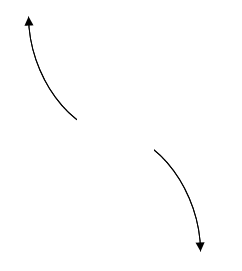
\includegraphics[width=0.3\textwidth]{../Figures/polyEndBehaviorCopyAC.png}
\end{center}\begin{enumerate}[label=\Alph*.]
\begin{multicols}{2}
\item 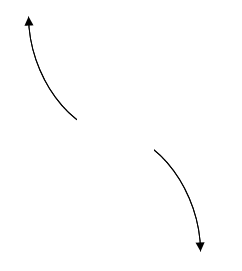
\includegraphics[width = 0.3\textwidth]{../Figures/polyEndBehaviorCopyAC.png}
\item 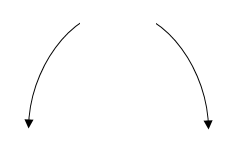
\includegraphics[width = 0.3\textwidth]{../Figures/polyEndBehaviorCopyBC.png}
\item 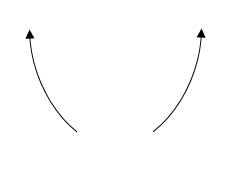
\includegraphics[width = 0.3\textwidth]{../Figures/polyEndBehaviorCopyCC.png}
\item 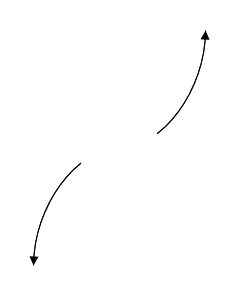
\includegraphics[width = 0.3\textwidth]{../Figures/polyEndBehaviorCopyDC.png}
\end{multicols}\item None of the above.\end{enumerate}
\textbf{General Comment:} Remember that end behavior is determined by the leading coefficient AND whether the \textbf{sum} of the multiplicities is positive or negative.
}
\litem{
Construct the lowest-degree polynomial given the zeros below. Then, choose the intervals that contain the coefficients of the polynomial in the form $ax^3+bx^2+cx+d$.
\[ \frac{7}{3}, \frac{-2}{5}, \text{ and } \frac{5}{3} \]
The solution is \( 45x^{3} -162 x^{2} +103 x + 70 \), which is option D.\begin{enumerate}[label=\Alph*.]
\item \( a \in [40, 47], b \in [157, 164], c \in [98, 105], \text{ and } d \in [-78, -62] \)

$45x^{3} +162 x^{2} +103 x -70$, which corresponds to multiplying out $(3x + 7)(5x -2)(3x + 5)$.
\item \( a \in [40, 47], b \in [10, 18], c \in [-187, -180], \text{ and } d \in [67, 80] \)

$45x^{3} +12 x^{2} -187 x + 70$, which corresponds to multiplying out $(3x + 3)(5x + 5)(3x -3)$.
\item \( a \in [40, 47], b \in [44, 51], c \in [-164, -157], \text{ and } d \in [-78, -62] \)

$45x^{3} +48 x^{2} -163 x -70$, which corresponds to multiplying out $(3x + 3)(5x -5)(3x -3)$.
\item \( a \in [40, 47], b \in [-162, -159], c \in [98, 105], \text{ and } d \in [67, 80] \)

* $45x^{3} -162 x^{2} +103 x + 70$, which is the correct option.
\item \( a \in [40, 47], b \in [-162, -159], c \in [98, 105], \text{ and } d \in [-78, -62] \)

$45x^{3} -162 x^{2} +103 x -70$, which corresponds to multiplying everything correctly except the constant term.
\end{enumerate}

\textbf{General Comment:} To construct the lowest-degree polynomial, you want to multiply out $(3x -7)(5x + 2)(3x -5)$
}
\litem{
Construct the lowest-degree polynomial given the zeros below. Then, choose the intervals that contain the coefficients of the polynomial in the form $x^3+bx^2+cx+d$.
\[ 5 + 3 i \text{ and } 1 \]
The solution is \( x^{3} -11 x^{2} +44 x -34 \), which is option B.\begin{enumerate}[label=\Alph*.]
\item \( b \in [-5, 2], c \in [-4, -1], \text{ and } d \in [2.3, 3.8] \)

$x^{3} + x^{2} -4 x + 3$, which corresponds to multiplying out $(x -3)(x -1)$.
\item \( b \in [-21, -10], c \in [43, 45], \text{ and } d \in [-36.5, -33.9] \)

* $x^{3} -11 x^{2} +44 x -34$, which is the correct option.
\item \( b \in [9, 16], c \in [43, 45], \text{ and } d \in [33.9, 36.3] \)

$x^{3} +11 x^{2} +44 x + 34$, which corresponds to multiplying out $(x-(5 + 3 i))(x-(5 - 3 i))(x + 1)$.
\item \( b \in [-5, 2], c \in [-9, -5], \text{ and } d \in [4.4, 5.8] \)

$x^{3} + x^{2} -6 x + 5$, which corresponds to multiplying out $(x -5)(x -1)$.
\item \( \text{None of the above.} \)

This corresponds to making an unanticipated error or not understanding how to use nonreal complex numbers to create the lowest-degree polynomial. If you chose this and are not sure what you did wrong, please contact the coordinator for help.
\end{enumerate}

\textbf{General Comment:} Remember that the conjugate of $a+bi$ is $a-bi$. Since these zeros always come in pairs, we need to multiply out $(x-(5 + 3 i))(x-(5 - 3 i))(x-(1))$.
}
\litem{
Describe the end behavior of the polynomial below.
\[ f(x) = 2(x + 7)^{3}(x - 7)^{4}(x - 3)^{4}(x + 3)^{6} \]
The solution is the graph below, which is option D.
\begin{center}
    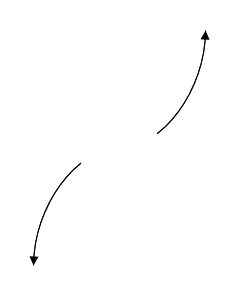
\includegraphics[width=0.3\textwidth]{../Figures/polyEndBehaviorDC.png}
\end{center}\begin{enumerate}[label=\Alph*.]
\begin{multicols}{2}
\item 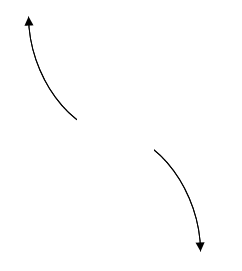
\includegraphics[width = 0.3\textwidth]{../Figures/polyEndBehaviorAC.png}
\item 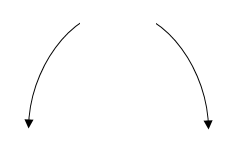
\includegraphics[width = 0.3\textwidth]{../Figures/polyEndBehaviorBC.png}
\item 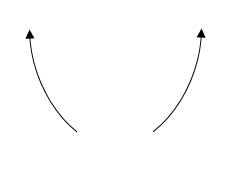
\includegraphics[width = 0.3\textwidth]{../Figures/polyEndBehaviorCC.png}
\item 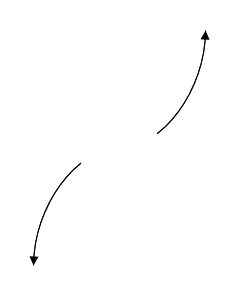
\includegraphics[width = 0.3\textwidth]{../Figures/polyEndBehaviorDC.png}
\end{multicols}\item None of the above.\end{enumerate}
\textbf{General Comment:} Remember that end behavior is determined by the leading coefficient AND whether the \textbf{sum} of the multiplicities is positive or negative.
}
\litem{
Which of the following equations \textit{could} be of the graph presented below?

\begin{center}
    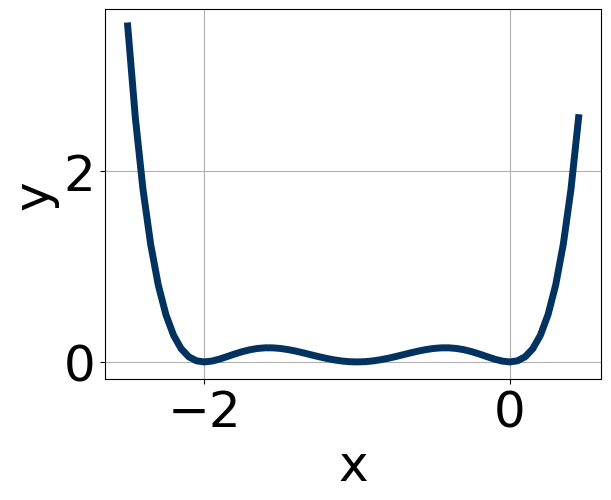
\includegraphics[width=0.5\textwidth]{../Figures/polyGraphToFunctionCopyC.png}
\end{center}



The solution is \( 20(x - 2)^{10} (x + 2)^{8} (x - 3)^{6} \), which is option B.\begin{enumerate}[label=\Alph*.]
\item \( -14(x - 2)^{6} (x + 2)^{8} (x - 3)^{6} \)

This corresponds to the leading coefficient being the opposite value than it should be.
\item \( 20(x - 2)^{10} (x + 2)^{8} (x - 3)^{6} \)

* This is the correct option.
\item \( -5(x - 2)^{10} (x + 2)^{10} (x - 3)^{5} \)

The factor $(x - 3)$ should have an even power and the leading coefficient should be the opposite sign.
\item \( 4(x - 2)^{8} (x + 2)^{6} (x - 3)^{5} \)

The factor $(x - 3)$ should have an even power.
\item \( 9(x - 2)^{8} (x + 2)^{11} (x - 3)^{5} \)

The factors $(x + 2)$ and $(x - 3)$ should both have even powers.
\end{enumerate}

\textbf{General Comment:} General Comments: Draw the x-axis to determine which zeros are touching (and so have even multiplicity) or cross (and have odd multiplicity).
}
\litem{
Which of the following equations \textit{could} be of the graph presented below?

\begin{center}
    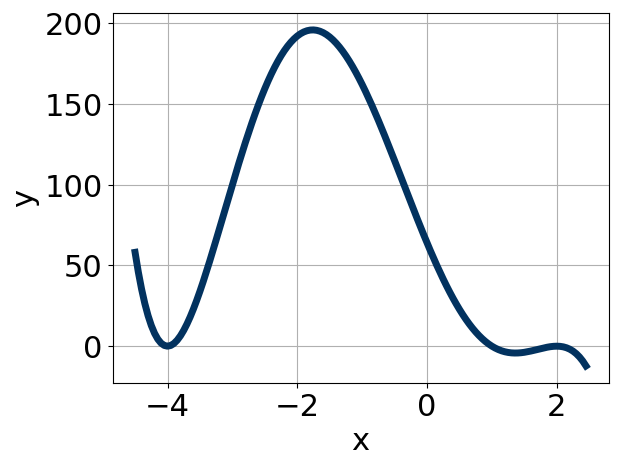
\includegraphics[width=0.5\textwidth]{../Figures/polyGraphToFunctionC.png}
\end{center}



The solution is \( -5x^{8} (x - 3)^{8} (x + 1)^{9} \), which is option C.\begin{enumerate}[label=\Alph*.]
\item \( 6x^{4} (x - 3)^{10} (x + 1)^{4} \)

The factor $(x + 1)$ should have an odd power and the leading coefficient should be the opposite sign.
\item \( 9x^{10} (x - 3)^{6} (x + 1)^{11} \)

This corresponds to the leading coefficient being the opposite value than it should be.
\item \( -5x^{8} (x - 3)^{8} (x + 1)^{9} \)

* This is the correct option.
\item \( -19x^{7} (x - 3)^{6} (x + 1)^{6} \)

The factor $x$ should have an even power and the factor $(x + 1)$ should have an odd power.
\item \( -10x^{11} (x - 3)^{4} (x + 1)^{9} \)

The factor $x$ should have an even power.
\end{enumerate}

\textbf{General Comment:} General Comments: Draw the x-axis to determine which zeros are touching (and so have even multiplicity) or cross (and have odd multiplicity).
}
\litem{
Construct the lowest-degree polynomial given the zeros below. Then, choose the intervals that contain the coefficients of the polynomial in the form $ax^3+bx^2+cx+d$.
\[ \frac{-7}{5}, 5, \text{ and } 2 \]
The solution is \( 5x^{3} -28 x^{2} +x + 70 \), which is option C.\begin{enumerate}[label=\Alph*.]
\item \( a \in [4, 9], b \in [-45, -40], c \in [95, 103], \text{ and } d \in [-73, -67] \)

$5x^{3} -42 x^{2} +99 x -70$, which corresponds to multiplying out $(5x + 5)(x -1)(x -1)$.
\item \( a \in [4, 9], b \in [22, 34], c \in [-8, 8], \text{ and } d \in [-73, -67] \)

$5x^{3} +28 x^{2} +x -70$, which corresponds to multiplying out $(5x -7)(x + 5)(x + 2)$.
\item \( a \in [4, 9], b \in [-34, -27], c \in [-8, 8], \text{ and } d \in [70, 73] \)

* $5x^{3} -28 x^{2} +x + 70$, which is the correct option.
\item \( a \in [4, 9], b \in [5, 9], c \in [-74, -67], \text{ and } d \in [70, 73] \)

$5x^{3} +8 x^{2} -71 x + 70$, which corresponds to multiplying out $(5x + 5)(x + 1)(x -1)$.
\item \( a \in [4, 9], b \in [-34, -27], c \in [-8, 8], \text{ and } d \in [-73, -67] \)

$5x^{3} -28 x^{2} +x -70$, which corresponds to multiplying everything correctly except the constant term.
\end{enumerate}

\textbf{General Comment:} To construct the lowest-degree polynomial, you want to multiply out $(5x + 7)(x -5)(x -2)$
}
\litem{
Describe the zero behavior of the zero $x = 9$ of the polynomial below.
\[ f(x) = 9(x + 9)^{6}(x - 9)^{9}(x - 3)^{5}(x + 3)^{7} \]
The solution is the graph below, which is option D.
\begin{center}
    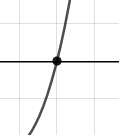
\includegraphics[width=0.3\textwidth]{../Figures/polyZeroBehaviorCopyDC.png}
\end{center}\begin{enumerate}[label=\Alph*.]
\begin{multicols}{2}
\item 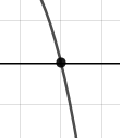
\includegraphics[width = 0.3\textwidth]{../Figures/polyZeroBehaviorCopyAC.png}
\item 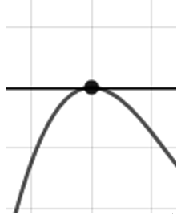
\includegraphics[width = 0.3\textwidth]{../Figures/polyZeroBehaviorCopyBC.png}
\item 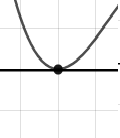
\includegraphics[width = 0.3\textwidth]{../Figures/polyZeroBehaviorCopyCC.png}
\item 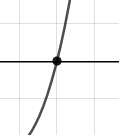
\includegraphics[width = 0.3\textwidth]{../Figures/polyZeroBehaviorCopyDC.png}
\end{multicols}\item None of the above.\end{enumerate}
\textbf{General Comment:} You will need to sketch the entire graph, then zoom in on the zero the question asks about.
}
\litem{
Construct the lowest-degree polynomial given the zeros below. Then, choose the intervals that contain the coefficients of the polynomial in the form $x^3+bx^2+cx+d$.
\[ 2 + 5 i \text{ and } 3 \]
The solution is \( x^{3} -7 x^{2} +41 x -87 \), which is option B.\begin{enumerate}[label=\Alph*.]
\item \( b \in [1, 2], c \in [-9.1, -7.3], \text{ and } d \in [10, 22] \)

$x^{3} + x^{2} -8 x + 15$, which corresponds to multiplying out $(x -5)(x -3)$.
\item \( b \in [-7, -4], c \in [40.5, 41.2], \text{ and } d \in [-93, -85] \)

* $x^{3} -7 x^{2} +41 x -87$, which is the correct option.
\item \( b \in [1, 2], c \in [-5.6, -1.6], \text{ and } d \in [3, 7] \)

$x^{3} + x^{2} -5 x + 6$, which corresponds to multiplying out $(x -2)(x -3)$.
\item \( b \in [6, 14], c \in [40.5, 41.2], \text{ and } d \in [87, 89] \)

$x^{3} +7 x^{2} +41 x + 87$, which corresponds to multiplying out $(x-(2 + 5 i))(x-(2 - 5 i))(x + 3)$.
\item \( \text{None of the above.} \)

This corresponds to making an unanticipated error or not understanding how to use nonreal complex numbers to create the lowest-degree polynomial. If you chose this and are not sure what you did wrong, please contact the coordinator for help.
\end{enumerate}

\textbf{General Comment:} Remember that the conjugate of $a+bi$ is $a-bi$. Since these zeros always come in pairs, we need to multiply out $(x-(2 + 5 i))(x-(2 - 5 i))(x-(3))$.
}
\litem{
Describe the zero behavior of the zero $x = -7$ of the polynomial below.
\[ f(x) = 2(x - 9)^{13}(x + 9)^{9}(x - 7)^{7}(x + 7)^{4} \]
The solution is the graph below, which is option C.
\begin{center}
    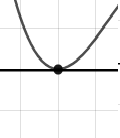
\includegraphics[width=0.3\textwidth]{../Figures/polyZeroBehaviorCC.png}
\end{center}\begin{enumerate}[label=\Alph*.]
\begin{multicols}{2}
\item 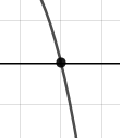
\includegraphics[width = 0.3\textwidth]{../Figures/polyZeroBehaviorAC.png}
\item 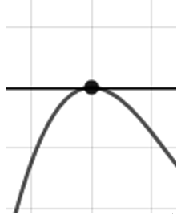
\includegraphics[width = 0.3\textwidth]{../Figures/polyZeroBehaviorBC.png}
\item 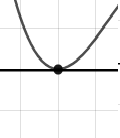
\includegraphics[width = 0.3\textwidth]{../Figures/polyZeroBehaviorCC.png}
\item 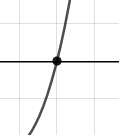
\includegraphics[width = 0.3\textwidth]{../Figures/polyZeroBehaviorDC.png}
\end{multicols}\item None of the above.\end{enumerate}
\textbf{General Comment:} You will need to sketch the entire graph, then zoom in on the zero the question asks about.
}
\end{enumerate}

\end{document}